\documentclass[12pt,a4psprt]{article}
\usepackage[spanish]{babel}
\usepackage[utf8]{inputenc}
\usepackage{eurosym}
\usepackage[pdftex]{graphicx}
\usepackage{listings}
\usepackage{bookmark}

\lstset{literate=
  {á}{{\'a}}1 {é}{{\'e}}1 {í}{{\'i}}1 {ó}{{\'o}}1 {ú}{{\'u}}1
  {Á}{{\'A}}1 {É}{{\'E}}1 {Í}{{\'I}}1 {Ó}{{\'O}}1 {Ú}{{\'U}}1
  {à}{{\`a}}1 {è}{{\`e}}1 {ì}{{\`i}}1 {ò}{{\`o}}1 {ù}{{\`u}}1
  {À}{{\`A}}1 {È}{{\'E}}1 {Ì}{{\`I}}1 {Ò}{{\`O}}1 {Ù}{{\`U}}1
  {ä}{{\"a}}1 {ë}{{\"e}}1 {ï}{{\"i}}1 {ö}{{\"o}}1 {ü}{{\"u}}1
  {Ä}{{\"A}}1 {Ë}{{\"E}}1 {Ï}{{\"I}}1 {Ö}{{\"O}}1 {Ü}{{\"U}}1
  {â}{{\^a}}1 {ê}{{\^e}}1 {î}{{\^i}}1 {ô}{{\^o}}1 {û}{{\^u}}1
  {Â}{{\^A}}1 {Ê}{{\^E}}1 {Î}{{\^I}}1 {Ô}{{\^O}}1 {Û}{{\^U}}1
  {œ}{{\oe}}1 {Œ}{{\OE}}1 {æ}{{\ae}}1 {Æ}{{\AE}}1 {ß}{{\ss}}1
  {ű}{{\H{u}}}1 {Ű}{{\H{U}}}1 {ő}{{\H{o}}}1 {Ő}{{\H{O}}}1
  {ç}{{\c c}}1 {Ç}{{\c C}}1 {ø}{{\o}}1 {å}{{\r a}}1 {Å}{{\r A}}1
  {€}{{\EUR}}1 {£}{{\pounds}}1 {ñ}{{\~n}}1 {Ñ}{{\~n}}1
}

\pagestyle{plain}
\title{\fbox{\fbox{\bf Práctica 1: Eficiencia}}}
\author{Antonio Jesús Heredia Castillo\\ 2ºA \\ ETS de Ingenierías Informática y de Telecomunicación }
\date{\today}
\begin{document}
%portada
\maketitle{}
	
\begin{abstract}
En esta practica obtendremos datos sobre el tiempo de ejecucion de distintos algoritmos y como afecta la compilacion al tiempo de ejecución.
\end{abstract}



%indice
\pagebreak
\tableofcontents                % Level 0 (chapter)
\pagebreak
\section{Sistema usado}
Para los ejercicios 1, 2, 3, 4 y 5 se ha usado el siguiente hardware:
\begin{center}
\begin{tabular}{|l||r|p{2cm}}
\hline
\multicolumn{2}{|c|}{Hardware} \\
\hline
CPU & Intel(R) Core(TM) i3-2310M\\
\hline
Velocidad de reloj & 2.10GHz \\
\hline
Arquitectura & 64bits \\
\hline
Memoria RAM & 5820 MiB \\
\hline
Tipo de maquina & x86\_64 \\
\hline

\end{tabular}
\end{center}

El sistema operativo usado a sido : \textbf{elementary OS Loki}.\\

Acontinuacion se adjunta una tabla con el hardware usado para los ejercicio 7.1, 7.2: \\
\begin{center}
\begin{tabular}{|l||r|p{2cm}}
\hline
\multicolumn{2}{|c|}{Hardware} \\
\hline
CPU & Intel(R) Core(TM) i5-6600 \\
\hline
Velocidad de reloj & 3.30GHz \\
\hline
Arquitectura & 64bits \\
\hline
Memoria RAM & 16GB \\
\hline
Tipo de maquina & x86\_64 \\
\hline

\end{tabular}
\end{center}

El sistema operativo usado a sido : \textbf{Linux Mint 18.1 Serena}.\\
Todos lo programas han sido compilados con g++ usando un nivel de optimizacion de 3.
\pagebreak
\section{Ejercicio 1: Ordenación de la burbuja}
\subsection{Codigo}
El codigo del programa principal es el siguiente:
\begin{lstlisting}[language=C++]
#include <iostream>
#include <ctime>    // Recursos para medir tiempos
#include <cstdlib>  // Para generación de números pseudoaleatorios

using namespace std;

void forma_usar(void){
	cerr << "Numero de parametro incorrecto" << endl;
	cerr << "Forma correcta de ejecutar: " << endl;
	cerr << "ejercicio7_1 tamaño valor_maximo" << endl;
	exit(1);
}

//Codigo copiado del PDF de practicas
void ordenar(int *v, int n) {
	for (int i=0; i<n-1; i++)
		for (int j=0; j<n-i-1; j++)
			if (v[j]>v[j+1]) {
			int aux = v[j];
			v[j] = v[j+1];
			v[j+1] = aux;
		}
}

int main(int argc, char * argv[])
{
  
	if (argc!=3)
		forma_usar();
	int tam=atoi(argv[1]);     // Tamaño del vector
	int max=atoi(argv[2]);    // Valor máximo
	
	if (tam<=0 || max<=0)
    	forma_usar();
  
	// Generación del vector aleatorio
	int *v=new int[tam];       // Reserva de memoria
	srand(time(0));            // Inicialización del generador de números pseudoaleatorios
	for (int i=0; i<tam; i++)  // Recorrer vector
		v[i] = rand() % max;    // Generar aleatorio [0,max[

	clock_t tini;    // Anotamos el tiempo de inicio
	tini=clock();

	ordenar(v,tam); // de esta forma forzamos el peor caso
  
	clock_t tfin;    // Anotamos el tiempo de finalización
	tfin=clock();

	// Mostramos resultados
	cout << tam << "\t" << (tfin-tini)/(double)CLOCKS_PER_SEC << endl;
  
  delete [] v;     // Liberamos memoria dinámica
}
\end{lstlisting}
\subsection{Eficiencia teorica}
La eficiencia teorica de la ordenacion burbuja podemos decir que es de:\\
$Eficiencia=\frac{n^{2}-2}{2}$
\pagebreak
\subsection{Representacion grafica}
La representacion de la eficiencia empirica de la ordenacion seria:
\begin{figure}[h]
\begin{center}
	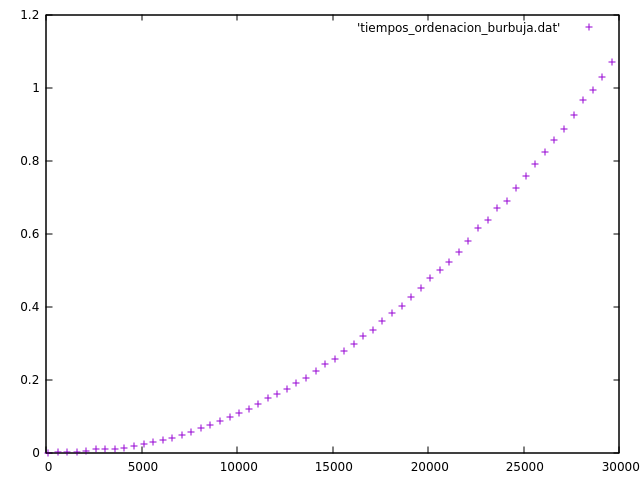
\includegraphics[scale=1]{image/grafica_1_sin_funcion.png}
\end{center}
\end{figure}
\\
En el siguiente grafico podemos ver como la eficiencia teorica
$f(x)=\frac{x^{2}-2}{2}$ junto a la eficiencia empirica.
\begin{figure}[h]
\begin{center}
	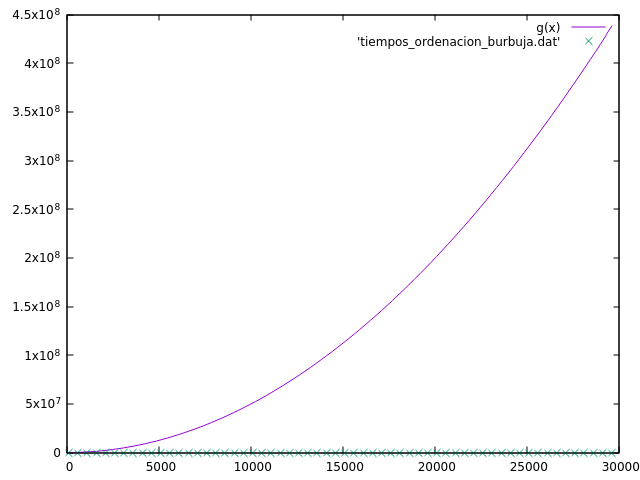
\includegraphics[scale=1]{image/grafica_1.png}
\end{center}
\end{figure}
\\
Con la eficiencia teorica sin ajustar, no se puede ver bien la curva de la eficiencia empirica.
\pagebreak
\section{Ejercicio 2: Ajuste en la ordenación de la burbuja}
Usando la herramient fit de gnuplot podemos ajustar los valores de una funcion para hacer que la eficiencia teorica conrresponda con la eficiencia empirica.
Para ello realizmos lo siguiente:
\begin{verbatim}
g(x) = a*x**2+b*x+c
fit g(x) 'tiempo_ordenacion_burbuja.data' via a,b,c
\end{verbatim}
Gnuplot ajustara g(x) a los tiempos obtenidos empiricamente y nos devuelve que $a=1.31596e-09$ , $b=-2.95575e-06$ y $c=0.00357733$. Cuando hagmamos un plot de la grafica y de g(x) conjuntamente obtenemos:
\begin{figure}[h]
\begin{center}
	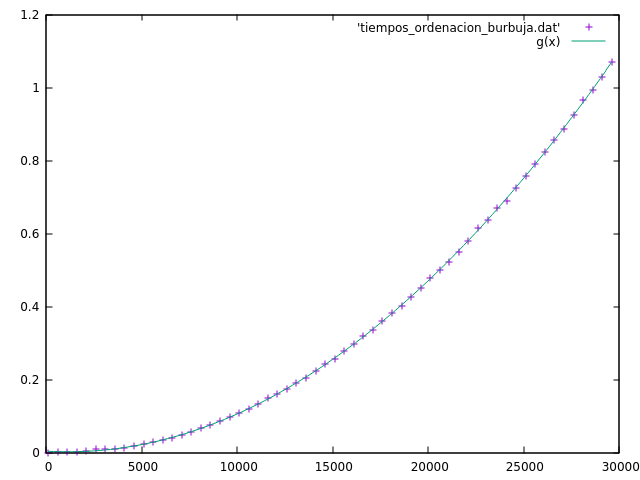
\includegraphics[scale=1]{image/grafica_2.png}
\end{center}
\end{figure}
\pagebreak
\section{Ejercicio 3: Problemas de precisión}
\subsection{Explique qué hace este algoritmo}
Consite en la busqueda de un elemento en un vector. Para ello el vector debe estar previamente ordenado.
El algoritmo divide el vector en dos partes, mira el elemento del medio, si el elemento a buscar es menor que el del medio, se queda con la parte izquierda del vector,
si es mayor, se queda con la derecha y si fuera igual, ya habria encontrado la posicion del elemento. Esto se ejecuta hasta que se encuentre el elemento.
\subsection{Calcule su eficiencia teórica}
Debido a que cada vez  se divide entre dos la region donde buscar, creo que la eficiencia teoria del algoritmo sera de \textbf{O(log(n))} .

\subsection{Calcule su eficiencia empirica}
Cuando se visualiza la eficiencia empirica podemos ver que todos los tados estan en el (0.0). Esto se debe a que el tiempo de ejecucion es tan pequeño que no lo podemos ni visualizar.\\ 
La solucion a este problema pasa por ejecutar el mismo algoritmo muchas veces y luego dividir el tiempo entre las veces que se ha ejecutado. En mi caso he ejecutado el algoritmo 10000 veces. Esto se podra observar en la siguiente seccion.\\
En la grafica podemos observar que los tiempos obtenidos se encuentran de forma escalonada. Esto se debe a la falta de precision a la hora de coger los datos. En este caso, f(x) no se consigue ajustar tan bien a los tiempos obtenidos, aunque si se puede observar que los datos si siguen la tendencia logaritmica.
\begin{figure}[h]
\begin{center}
	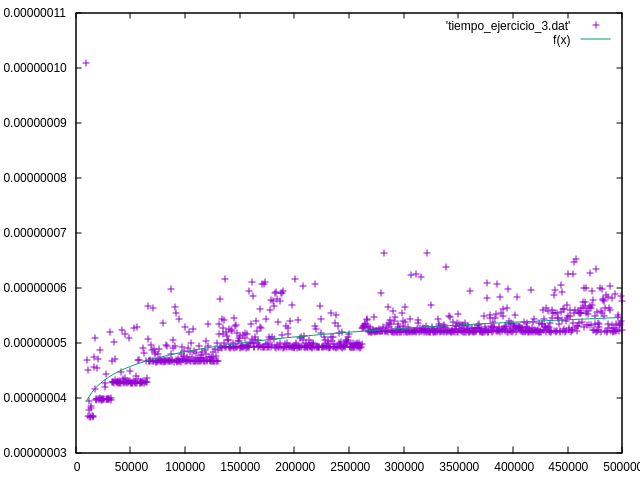
\includegraphics[scale=1]{image/grafica_3.png}
\end{center}
\end{figure}
\pagebreak
\subsection{Codigo}
\begin{lstlisting}{language=C++}
#include <iostream>
#include <ctime>    // Recursos para medir tiempos
#include <cstdlib>  // Para generación de números pseudoaleatorios

using namespace std;

int operacion(int *v, int n, int x, int inf, int sup) {
  int med;
  bool enc=false;
  while ((inf<sup) && (!enc)) {
    med = (inf+sup)/2; 
    if (v[med]==x) 
      enc = true;
    else if (v[med] < x) 
      inf = med+1;
    else
      sup = med-1;
  }
  if (enc) 
    return med;
  else 
    return -1;
}

void sintaxis()
{
  cerr << "Sintaxis:" << endl;
  cerr << "  TAM: Tamaño del vector (>0)" << endl;
  cerr << "Se genera un vector de tamaño TAM con elementos aleatorios" << endl;
  exit(EXIT_FAILURE);
}

int main(int argc, char * argv[])
{
  // Lectura de parámetros
  if (argc!=2)
    sintaxis();
  int tam=atoi(argv[1]);     // Tamaño del vector
  if (tam<=0)
    sintaxis();
  
  // Generación del vector aleatorio
  int *v=new int[tam];       // Reserva de memoria
  srand(time(0));            // Inicialización del generador de números pseudoaleatorios
  for (int i=0; i<tam; i++)  // Recorrer vector
    v[i] = rand() % tam;
  
  clock_t tini;    // Anotamos el tiempo de inicio
  tini=clock();

  // Algoritmo a evaluar
  for(int x = 0; x < 10000; x++) // Se realiza 10000 para obtener tiempos adecuados
    operacion(v,tam,tam+1,0,tam-1);
  
  clock_t tfin;    // Anotamos el tiempo de finalización
  tfin=clock();

  // Mostramos resultados
  cout << tam << "\t" << (tfin-tini)/(double)CLOCKS_PER_SEC/10000 << endl;
  
  delete [] v;     // Liberamos memoria dinámica
}

\end{lstlisting}
\section{Ejercicio 4: Mejor y peor caso}
Para el peor caso posible lo que he realizado es llenar el vector de la siguiente forma:
\begin{lstlisting}
	int cont_inverso = tam;
	for (int i=0; i<tam; i++){
		v[i] = cont_inverso;    // ordenados de forma inversa
		cont_inverso--;
	}  // Recorrer vector

\end{lstlisting}
Y para obtener el mejor caso posible lo he realizado asi:
\begin{lstlisting}

	for (int i=0; i<tam; i++)
		v[i] = i;    // ordenados
\end{lstlisting}
La grafica que obtenemos al ejecutar los diferentes codigos es:
\begin{figure}[h]
\begin{center}
	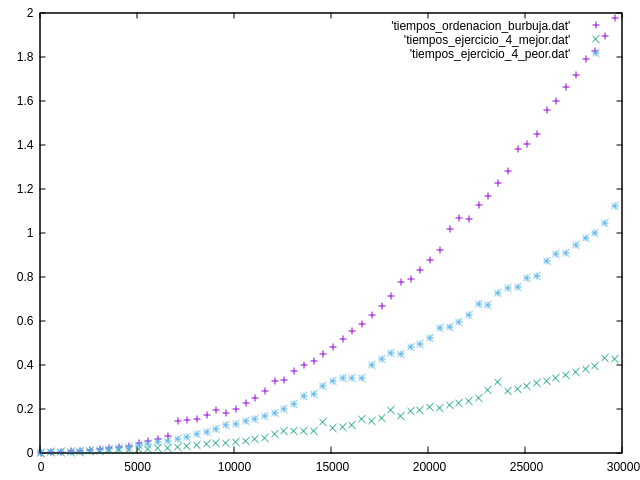
\includegraphics[scale=1]{image/grafica_4.png}
\end{center}
\end{figure}
\section{Ejercicio 5: Dependencia de la implementacion}
En la implementacion del algoritmo burbuja que nos dan en este ejercicio y suponiendo que nos encontramos en el mejor caso posible. El algoritmo tendra una eficiencia de \textbf{O(n)}.
\\Esto se debe a que solo realizara una pasada al vector, porque cuando en la primera pasada, no haya realizado ningun cambio, no volvera a relizar ninguna pasada mas el bucle. Consiguiendo asi una eficiencia lineal.
\begin{figure}[h]
\begin{center}
	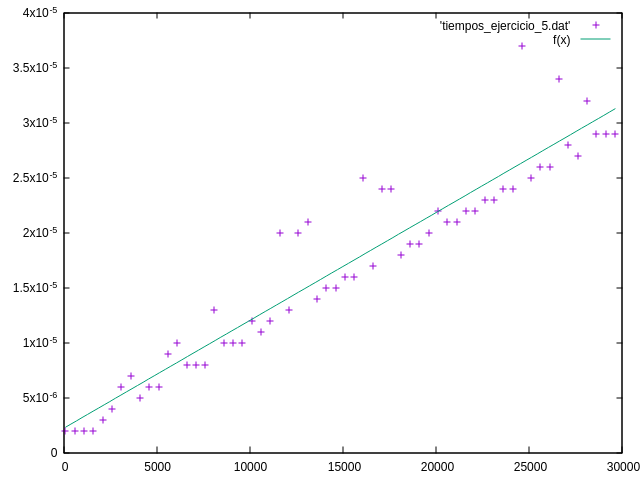
\includegraphics[scale=1]{image/grafica_5.png}
\end{center}
\end{figure}
\\
El ejercicio 3,4,5 los he realizado en un PC con pocos recursos y por ello, a la hora de recoger los datos, no he obtenido siempre buenos resultados y por ello creo que la f(x) no se ajusta adecuadamente a la linea de puntos. Pero si que se puede observar que si siguen la misma tendencia.
\section{Ejercicio 7.1: Dependencia del entorno}
\subsection{Codigo}
El codigo del programa principal es el siguiente:
\begin{lstlisting}[language=C++]
#include <iostream>
#include <ctime>    // Recursos para medir tiempos
#include <cstdlib>  // Para generacion de numeros pseudoaleatorios
using namespace std;

void forma_usar(void){
	cerr << "Numero de parametro incorrecto" << endl;
	cerr << "Forma correcta de ejecutar: " << endl;
	cerr << "ejercicio7_1 tamaño valor_maximo" << endl;
	exit(1);
}

//Codigo copiado del PDF de practicas
void ordenar(int *v, int n) {
	bool cambio=true;
	for (int i=0; i<n-1 && cambio; i++) {
		cambio=false;
		for (int j=0; j<n-i-1; j++)
			if (v[j]>v[j+1]) {
				cambio=true;
				int aux = v[j];
				v[j] = v[j+1];
				v[j+1] = aux;
			}
	}
}

int main(int argc, char * argv[])
{
	if (argc!=3)
		forma_usar();
	int tam=atoi(argv[1]);     // Tamaño del vector
	int max=atoi(argv[2]);    // Valor maximo
	
	if (tam<=0 || max<=0)
    	forma_usar();
  
	// Generacion del vector aleatorio
	int *v=new int[tam];       // Reserva de memoria.
	// Inicializacion del generador de numeros pseudoaleatorios
	srand(time(0));            
	for (int i=0; i<tam; i++)  // Recorrer vector
		v[i] = rand() % max;    // Generar aleatorio [0,max[

	clock_t tini;    // Anotamos el tiempo de inicio
	tini=clock();

	ordenar(v,tam); // de esta forma forzamos el peor caso
  
	clock_t tfin;    // Anotamos el tiempo de finalizaciun
	tfin=clock();

	// Mostramos resultados
	cout << tam << "\t" << (tfin-tini)/(double)CLOCKS_PER_SEC 
	<< endl;
  
  delete [] v;     // Liberamos memoria dinamica
}

\end{lstlisting}

\pagebreak
Apartir de los datos obtenidos  podemos realizar una grafica para ver si la eficiencia teoria que en este caso seria O($n^{2}$) corresponde con la eficiencia empirica. Donde la funcion tendria la siguiente forma: \textbf{$f(x)=a*x^{2}+b $}
\begin{figure}[h]
\begin{center}
	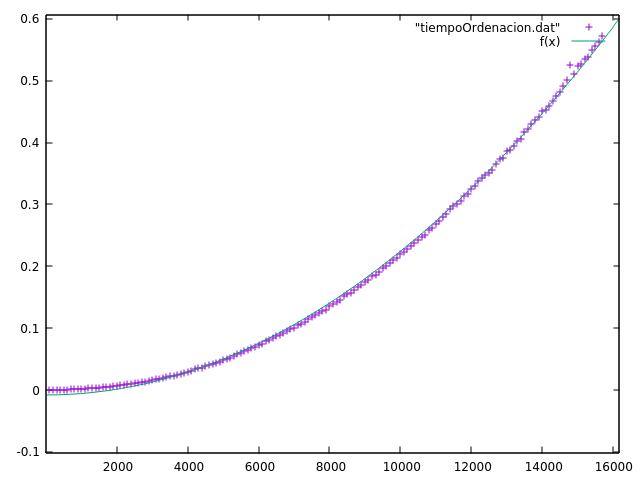
\includegraphics[scale=1]{image/grafica_7_1.png}
\end{center}
\caption{Grafica ejercicio 7.1}

\end{figure}
\\
Gracias a gnuplot podemos obtener el ajuste para a y b en f(x) para los datos obtenidos.
He obtenido que $a=-2.32*10^{-9}$ y $b=-0.0079$
\section{Ejercicio 7.2: Multiplicación matricial}

\subsection{Codigo}
El codigo del programa principal es el siguiente:
\begin{lstlisting}[language=C++]
#include <iostream>
#include <ctime>    // Recursos para medir tiempos
#include <cstdlib>  // Para generación de números pseudoaleatorios

using namespace std;

void forma_usar(void){
	cerr << "Numero de parametro incorrecto" << endl;
	cerr << "Forma correcta de ejecutar: " << endl;
	cerr << "ejercicio7_2 tamaño " << endl;
	exit(1);
}

void multiplicar(int **m1, int **m2, int **m3, int tam) {
	
	for(int c = 0; c < tam; c++)
		for(int f = 0; f < tam; f++){
			int suma = 0;
			
			for(int x = 0; x < tam; x++)
				suma += m1[f][x]*m2[c][x];

			m1[f][c] = suma;
		}
			
	
}

int main(int argc, char * argv[])
{
  
	if (argc!=3)
		forma_usar();
	int tam=atoi(argv[1]);     // Tamaño de la matriz
	int max=atoi(argv[2]);

	if (tam<=0)
    	forma_usar();


	int **matriz1;
	int **matriz2;
	int **matriz3;

  	matriz1 = new int * [tam];
	matriz2 = new int * [tam];
	matriz3 = new int * [tam];

	for(int f = 0; f < tam; f++){
		matriz1[f] = new int  [tam];
		matriz2[f] = new int  [tam];
		matriz3[f] = new int  [tam];
	
	}
 	// Inicialización del generador de números pseudoaleatorios
	srand(time(0));           
	for(int f = 0; f < tam; f++)
		for(int c = 0 ; c < tam; c++){
			matriz1[f][c] = rand() % max; 
			matriz2[f][c] = rand() % max; 
		}
	

	clock_t tini;    // Anotamos el tiempo de inicio
	tini=clock();

	multiplicar(matriz1, matriz2, matriz3, tam);
	
	clock_t tfin;    // Anotamos el tiempo de finalización
	tfin=clock();

	// Mostramos resultados
	cout << tam << "\t" 
	<< (tfin-tini)/(double)CLOCKS_PER_SEC << endl;
  
	for(int f = 0; f < tam; f++){
		delete matriz1[f];
		delete matriz2[f];
		delete matriz3[f];
	}     // Liberamos memoria dinámica
	
	delete matriz1;
	delete matriz2;
	delete matriz3;
	
}

\end{lstlisting}
\pagebreak
En este caso la eficiencia teorica seria O($n^{3}$) y por lo tanto no se puede ajustar correctamente con una funcion del estilo: \textbf{$f(x)=a*x^{2}+b $}.
\begin{figure}[h]
\begin{center}
	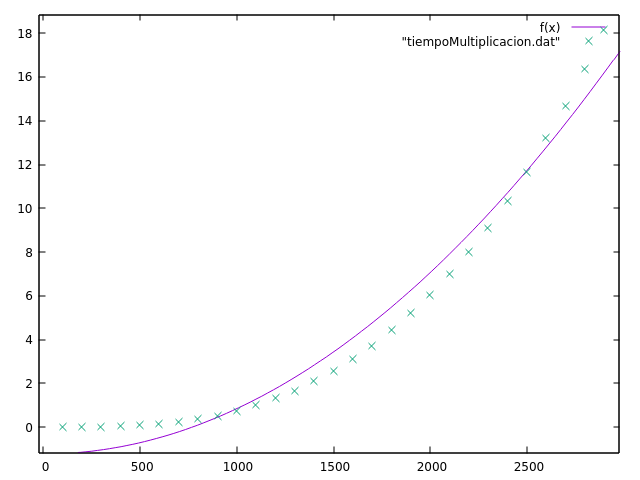
\includegraphics[scale=1]{image/grafica_7_2_cuadratica.png}
\end{center}
\caption{Grafica ejercicio 7.2 cuadratica}
\end{figure}
\\Como podemos obserbar la linea de f(x) en este caso no se ajusta de forma exacta a la nube de puntos de los datos que hemos obtenido.\\
\pagebreak
\\En cambio con \textbf{$f(x)=a*x^{3}+b $} si que se ajustaria bien la eficiencia teoriaca con la eficiencia empirica.\\.

\begin{figure}[h]
\begin{center}
	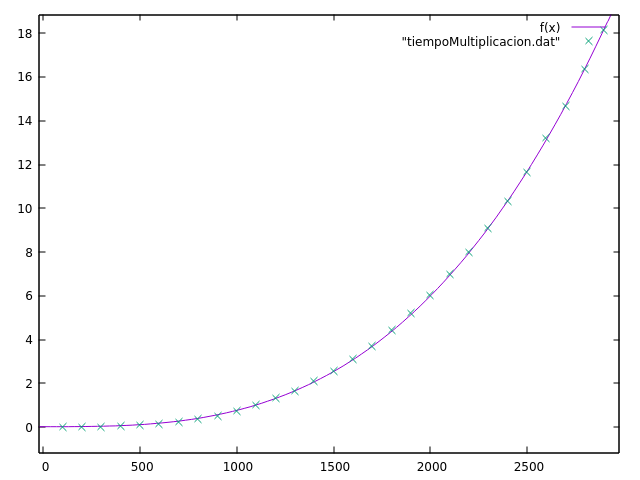
\includegraphics[scale=1]{image/grafica_7_2_cubica.png}
\end{center}
\caption{Grafica ejercicio 7.2 cubica}

\end{figure}



\end{document}